\documentclass[11pt, a4paper]{article}
\usepackage{minted}
\usepackage{tikz}
\usepackage{tabu}


\title{Houston}
\usetikzlibrary{er,positioning}
 
\begin{document}

\maketitle
	
	
\begin{abstract}
Houston can be described as a mission control tool for robotic systems with the extended functionalities of generating and analyzing tests. The current version of Houston focuses on Arducopter an open-source multi UAV controller. The need for a tool such as Houston arises when contemplating how bad humans are at creating tests, specially for robots.
\end{abstract}
	
	
\section{Introduction}
Houston is a mission control tool for robotic systems with the extended features of generating and analyzing tests. Houston is a key part of our main goal of automatically generating high-quality test suites for robotic systems. Houston uses ROS (Robot Operating System) a framework for developing robotic applications. In the case of ArduCopter, Houston works directly with MAVROS a ROS node that works as a ground control station. Houston can be executed in two ways, the first by passing a JSON file with a mission description, and the second by letting it randomly generate a mission. \footnote{This might not be completely true, since we do have to give Houston some limitations for the test generator}  The layout of this paper is as follow: Section 1.1 briefly describes ArduCopter. Sections 2 presents mission parameters, Section 3 describes how Houston work, section 4 looks into the output data and section 5 presents future work. 


\section{Mission Parameters}
\paragraph{}
Mission parameters are a set of values that represent the expected behavior of a system. Such values can change depending in the mission type. Our goal is to be as flexible as possible. We have accounted for robot type, launch file \footnote{not so much for ArduCopter but it can be expanded to work with}, map, and the mission type which describes the mission in detail.


\subsection{JSON input}
Houston is enabled to receive as input a JSON file containing mission specifications such as intents, quality attributes, failure flags and action descriptions for the robot to accomplish. An example for an action would be point to point which is basically an instruction for the robot to go to another location. The following is an example of a JSON file containing mission specifications.
\begin{minted}
[fontsize=\scriptsize,
baselinestretch=1,
framesep=1mm]
{json}
{
	"MDescription":
	{
		"RobotType":	"ArduCopter",
		"LaunchFile":	"robotest.launch",
		"Map":	"Airport.world",
		"Mission":
		{
			"Name":"JustARide",
			"Action":
			{
				"Type": "PTP",
				"alt" : "5.0",
				"x":	"0.0",
				"y":	"0.0",
				"z":	"5.0",
				"x_d":	"0.0",
				"y_d":	"0.0",
				"z_d":	"0.0"
			},
			"QualityAttributes":
			{
				"ReportRate":"2",
				"Time": "True",
				"Battery": "False",
				"MaxHeight": "True",
				"MinHeight": "True"
			},
			
			"Intents":
			{
				"Time": "10",  
				"Battery": ".6",  
				"MaxHeight": "20",  
				"MinHeight": "10"
			},
			
			"FailureFlags":
			{
				"Time":	"40.0",
				"Battery": "90",
				"SystemShutdown":"True",
				"MaxHeight":      "30",
				"MinHeight":      "20"
			}
			
		}
		
	}
}
\end{minted}

 
\subsection{Quality Attributes}
\paragraph{}
Having data available regarding the performance of the system allows us to understand the system and its mission performance. It can also provide us with some needed data for the later development of automatic semi-directed test generation. Some examples of quality attributes are:
\begin{itemize}
	\itemsep-.5em
	\item Time taken
	\item Power consumption 
	\item Max height 
	\item Min height (previous to land command)
	\item ...		
\end{itemize}

\subparagraph{}
More quality attributes to be added as we discover more interesting properties.

\subsection{Intents}
\paragraph{}
Intents are expectations for the system under test. Intents can vary depending on the given mission. They can also bound a mission. For example if a given system exceeds a marked height, the final report marks such an event as a ``unmet intent". Providing the mission with intents can help us later generate better tests for the system (as with quality attributes). Example for intents are:
\begin{itemize}
	\itemsep-.5em
	\item Finish in a given time frame
	\item Finish using less than a given percentage of battery  
	\item Boundaries in height (previous to land command)
	\item ...		
\end{itemize}
\subparagraph{}
More quality attributes will added as we discover more interesting properties

\subsection{Failure Flags}
\paragraph{}
As with intents, failure flags bound a mission, with the difference that if such ``intent" is unmet, the mission stops and immediately marks the test as failed.  

\subsection{Missions}
We now present three missions. We use JSON files to pass all the mission information to Houston which executes and monitors the mission.
\subsubsection{Point to Point (PTP)}
A simple but necessary mission is “point to point” which commands the system to start at a given location then move to another position.
\subsubsection{Multiple Point to Point (MPTP)}
Similar to PTP, MPTP is a simple mission where there are multiple locations for the system to visit. It can be described as a collection of PTPs. This mission can help us study the performance of the system under different altitudes.
\subsubsection{Extraction}
Similar to PTP, in the “extraction” mission, the system goes to a given location, lands, waits a set amount of time, then returns to its starting position.
\section{Houston Under the Hood }
\paragraph{}
We now present how Houston actually works. The structure of Houston can be divided in architecture, sending commands, verifying command completion, mission monitor and generating reports. In section 3.1 we look into how Houston relates with the testing environment. In sections 3.2 and 3.3 we show how Houston sends commands and how it verifies the completion of such. Houston constantly monitors the system and the mission progress, we present how it works in section 3.4. In section 3.5 we show how Houston generates reports. 
\subsection{Enviroment Architecture}
In the specific case of ArduPilot Houston requires \footnote{Gazebo is not a need, but it does help visualize the test. It can also add more variation to the tests by having different maps (worlds).} the following programs to be running:
\begin{itemize}
 	\itemsep-.5em
 	\item ArduCopter
 	\item Gazebo
 	\item ROS (roscore)
 	\item MAVROS (Ground control node)
\end{itemize}
Houston receives all the data related to the simulation from mavros which requires roscore to the running. AduCopter is the system that we want to study, for the most part we run it along side with Gazebo a 3D modeler for simulations. Gazebo allows to see missions in progress and study the behavior of the system. More than that by using Gazebo we can model our own worlds and then test ArduCopter with it. 
\begin{figure}
\begin{center}
	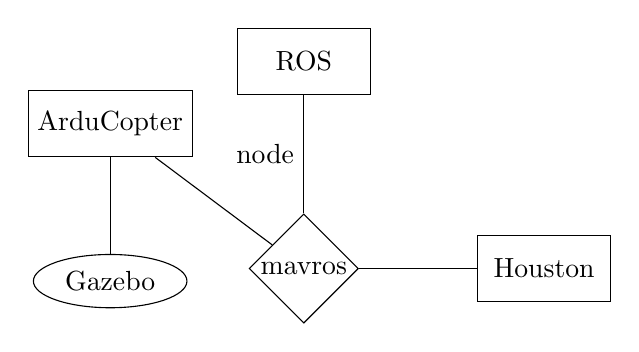
\begin{tikzpicture}[auto,node distance=1.5cm]
	
	% Create an entity with ID node1, label "Fancy Node 1".
	% Default for children (ie. attributes) is to be a tree "growing up"
	% and having a distance of 3cm.
	%
	% 2 of these attributes do so, the 3rd's positioning is overridden.
	\node[entity] (node1) {ArduCopter}
	[grow=up,sibling distance=3cm]
	
	child[grow=down,level distance=2cm] {node[attribute] {Gazebo}};
	% Now place a relation (ID=rel1)
	\node[relationship] (rel1) [below right = of node1] {mavros};
	% Now the 2nd entity (ID=rel2)
	\node[entity] (node2) [above  = of rel1]	{ROS};
	
	\node[entity] (node3) [ right = of rel1]	{Houston};
	% Draw an edge between rel1 and node1; rel1 and node2
	\path (rel1) edge node {} (node1)
	 edge	 node {node}	(node2);
	\path (rel1) edge node {} (node3);
	
	\end{tikzpicture}
\end{center}
 \caption{Environment Architecture}
 \label{EnvironmentArchitecture}
\end{figure}
In figure Figure~\ref{EnvironmentArchitecture} we can see the relation that each program has with the others. Mavros takes the role of being the link of communication between the targeted system (ArduCopter) and Houston. We can also appreciate how Gazebo is a non-essential part for testing. 

\subsection{Sending Commands}
In the previous section we pointed out how mavros was the link of communication between the targeted system and Houston. Houston communicates with mavros in two ways, the first by using services and second by publishing topics. We now give a brief description of what services and topics are in relation to ROS and how they are used by Houston.
\subsubsection{Services}
Services are a method of communication in ROS. They are used for bi-directional transmission of data. Node x can call node y, and node y can call node x. Houston uses services to set flying modes, arm the quadcopter, takeoff and land. Service calls are usually presented as remote procedure calls. In Table~\ref{HoustonServices} we show the services being used and their types.

\begin{table}
\begin{tabu} to 0.0\textwidth { | X[l]| X[l] | X[l] | }
	\hline
	ID & Service & Type \\
	\hline
	\hline
	1  & /mavros/set\_mode  & SetMode  \\
	\hline
	2  & /mavros/cmd/arming & CommandBool \\
	\hline
	3  & /mavros/cmd/takeoff & CommandTOL \\
	\hline
\end{tabu}
 \caption{Services used by Houston}
 \label{HoustonServices}
\end{table}
Service 1 is called to set the flight mode of the quadcopter to guided. Guided mode allows Houston to send locations for the system to visit. Service 2 is called to arm the system motors, and service 3 is called to command the quadcopter to takeoff. Service 3 receives as a  parameter a desired altitude.   
\subsubsection{Topics}
Topics are also another method of communication in ROS. Nodes that use topics as a form of communication are unaware of the end side, meaning that they do not know if another node is receiving data. It is possible to subscribe or to publish a topic. Nodes subscribe to a topic to receive data and publish when the goal is to send data. Houston uses topics to receive information of the system and to send locations for the system to visit. In Table~\ref{HoustonTopics} we show the topics being used by Houston. Topic 4 is used to send positions for the quadcopter to visit, it takes as parameters x, y, and z. 

\begin{table}
	\begin{tabular} {|p{.4cm} |p{5.5cm}|p{3cm}|p{4cm}|}
		\hline
		ID & Topic & Type & Pub/Sub \\
		\hline
		\hline
		1  & /mavros/local\_position/pose  & PoseStamped  & Subscribes \\ 
		\hline
		2  & /mavros/global\_position/global & NavSatFix & Subscribes \\
		\hline
		3  & /mavros/battery & BatteryStatus & Subscribes \\ 
		\hline
		4  & /mavros/local\_position/odom & Odometry & Subscribes \\
		\hline
		5 & /mavros/setpoint\_position/local &  PoseStamped & Publishes \\
		
		\hline
	\end{tabular}
	\caption{Topics used by Houston}
	\label{HoustonTopics}
\end{table}

\subsection{Verifying Command Completion}
Previously we said that topics are a one-way communication method. This means that if we tell the system to go to a location we can not really tell if the system reached the goal. We have worked around this by not only publishing the location we want the system to go to but also subscribing to topics 1, 3 and 4 (Table~\ref{HoustonTopics}) which keeps us updated of the current position. To verify the correct completion of a point to point task Houston has two ways of accomplishing this. Since the whole idea is to test robotic systems, we do not want to only rely on one source of data.
\subsubsection{Using Local Position (Odometry)}
Topic 4 provides Houston the current x, y and z local positions, these values are given meters. Then by finding the distance between the current location and the desired location we can tell if the system has reached its goal. 
\begin{minted}
[fontsize=\footnotesize,
baselinestretch=1,
framesep=1mm]
{python}
while euclidean((current_position),(target_position)) > 0:
	mavros_local_odom_publisher.publish(target_locaiton)
\end{minted}

\subsubsection{Using Coordinates (Latitude \& Longitude)}
Assuming that we do not have access to topic 4 and no values for our current x, y and z positions, Houston has to work around it by using Latitude and Longitude which are given by topic 2. Houston has as constants the values for home (0,0) in latitude and longitude (-35.3632607, 149.1652351) which is the starting position of the system (this specific build of ArduCopter). This approach looks into checking the distance between two coordinates instead of two points (x and y). In this specific case x represents the longitude and y the latitude. We find the current x by measuring the distance between the current longitude and the constant home longitude, if the home longitude is greater than the current longitude then x is turn into negative. We find y with the same procedure, only that we use latitude.
\begin{minted}
[fontsize=\scriptsize,
baselinestretch=1,
framesep=1mm]
{python}
x = great_circle(HOME_COORDINATES, (HOME_COORDINATES[0], current_global_coordinates[1],))
y = great_circle(HOME_COORDINATES, (current_global_coordinates[0], HOME_COORDINATES[1],))
if HOME_COORDINATES[0]> current_global_coordinates[0]:
	y *= -1
if HOME_COORDINATES[1]> current_global_coordinates[1]:
	x *= -1
        
return x, y
\end{minted}
Houston can now generate an expected coordinate using the systems current x and y values. First it finds how much it has to add or subtract to the latitude and longitude. It finds the horizontal increment by finding the distance between the current y and the target y, then it does the same for the vertical increment, instead of y it uses x.
\begin{minted}
[fontsize=\scriptsize,
baselinestretch=1,
framesep=1mm]
{python}

earth_radius = 6378000.0 

if target_y > current_y:
    expected_lat  = initial_global_lat + ((y_increment / earth_radius) * (180.0/math.pi))
else:
    expected_lat  = initial_global_lat - ((y_increment / earth_radius) * (180.0/math.pi))
if target_x > current_x:
    expected_long = initial_global_long + ((x_increment / earth_radius) * (180.0/math.pi)/ 
    math.cos(math.radians(initial_global_lat)))
else:
    expected_long = initial_global_long - ((x_increment / earth_radius) * (180.0/math.pi)/ 
    math.cos(math.radians(initial_global_lat)))

return expected_lat, expected_long
\end{minted}
Now that we have an expected coordinate and a current coordinate Houston checks how close the system is to its goal and says if the expected location is reached. 


\subsection{Mission Monitor}
By subscribing to topics 1, 2, 3, and 4 Houston has live data about the systems battery, local and global position. Houston uses the local position keep record of the maximum and minimum height. The systems battery data is used to measure the total battery used for a mission. The distance traveled is measured using the global position data. Having all this data available the mission monitor checks for intents, failure flags and quality attributes. Then it generates reports about the performance of the system on a given mission. 
\subsection{Generating Reports}
Reports are given in JSON format, an example of a report is the following:
\begin{minted}
[fontsize=\scriptsize,
baselinestretch=1,
framesep=1mm]
{python}

earth_radius = 6378000.0 

if target_y > current_y:
expected_lat  = initial_global_lat + ((y_increment / earth_radius) * (180.0/math.pi))
else:
expected_lat  = initial_global_lat - ((y_increment / earth_radius) * (180.0/math.pi))
if target_x > current_x:
expected_long = initial_global_long + ((x_increment / earth_radius) * (180.0/math.pi)/ 
math.cos(math.radians(initial_global_lat)))
else:
expected_long = initial_global_long - ((x_increment / earth_radius) * (180.0/math.pi)/ 
math.cos(math.radians(initial_global_lat)))

return expected_lat, expected_long
\end{minted}

\section{Understanding Reports}
An example of a report is:
\begin{minted}
[fontsize=\scriptsize,
baselinestretch=1,
framesep=1mm]
{json}
{
    "MissionType": "PTP", 
    "Intents": {
    "Battery": true, 
    "MinHeight": {"MinHeight": 0.5266779065132147, "Success": false, "Time": 39.99999499320984}, 
    "MaxHeight": true, 
    "Time": {"Success": false, "Time": 39.99999499320984}
    }, 
    "OverallTime": "40.0000100136", 
    "Failure Flags": "Time exceeded", 
    "Map": "Airport.world", 
    "LaunchFile": "robotest.launch", 
    "RobotType": "ArduCopter", 
    "QualityAttributes": [
        {"Battery": 0.0, "MinHeight": -1, "MaxHeight": 0, "Time": 2.141758}, 
        {"Battery": 0.0, "MinHeight": -1, "MaxHeight": 0.0075184097, "Time": 4.14176702}, 
        {"Battery": 0.0, "MinHeight": -1, "MaxHeight": 0.0110572380, "Time": 6.14323806}, 
        {"Battery": 0.009999997, "MinHeight": -1, "MaxHeight": 1.0763062238693237, "Time": 8.1432418}, 
        {"Battery": 0.009999997, "MinHeight": -1, "MaxHeight": 3.9529566764831543, "Time": 10.143244}, 
        {"Battery": 0.019999995, "MinHeight": 4.8817729, "MaxHeight": 5.08878231, "Time": 12.143249}, 
        {"Battery": 0.019999995, "MinHeight": 4.8817729, "MaxHeight": 5.09394884, "Time": 14.143256}, 
        {"Battery": 0.029999993, "MinHeight": 4.8817729, "MaxHeight": 5.09394884, "Time": 16.143260}, 
        {"Battery": 0.02999999, "MinHeight": 4.88177299, "MaxHeight": 5.09394884, "Time": 18.143264}, 
        {"Battery": 0.039999991, "MinHeight": 4.8817729, "MaxHeight": 5.09394884, "Time": 20.143265}, 
        {"Battery": 0.039999991, "MinHeight": 4.8817729, "MaxHeight": 5.09394884, "Time": 22.143270}, 
        {"Battery": 0.049999997, "MinHeight": 4.8817729, "MaxHeight": 5.09394884, "Time": 24.143284}, 
        {"Battery": 0.049999997, "MinHeight": 4.8817729, "MaxHeight": 5.09394884, "Time": 26.143290}, 
        {"Battery": 0.059999994, "MinHeight": 4.8817729, "MaxHeight": 5.09394884, "Time": 28.143296}, 
        {"Battery": 0.059999994, "MinHeight": 4.8817729, "MaxHeight": 5.09394884, "Time": 30.143302}, 
        {"Battery": 0.069999996, "MinHeight": 4.8817729, "MaxHeight": 5.09394884, "Time": 32.143764}, 
        {"Battery": 0.069999996, "MinHeight": 4.8817729, "MaxHeight": 5.09394884, "Time": 34.143770}, 
        {"Battery": 0.079999996, "MinHeight": 4.8817729, "MaxHeight": 5.09394884, "Time": 36.143776}, 
        {"Battery": 0.079999994, "MinHeight": 4.8817729, "MaxHeight": 5.09394884, "Time": 38.143781}]
}
\end{minted}

...
\section{Future}
...



	
\end{document}
